\documentclass{article}
\usepackage[en]{ukon-infie}
\usepackage[utf8]{inputenc}
\usepackage{algorithm2e}
\usepackage{amsmath}
\usepackage{graphicx}
% kann de oder en sein
% kann bubble break, topexercise sein

\Names{Jonas Probst, Simon Giebenhain}
\Lecture[AnaVis]{Analyse und Visualisierung von Informationen}
\Term{WS 2017/18}

\begin{document}
    \begin{ukon-infie}[12.12.17]{7}

        \begin{exercise}[p=7]{Single/Average Linkage}      

		\end{exercise}
		
		\begin{exercise}[p=2]{DENCLUE}
		$\xi=0$\\
		Center defined clusters.\\
		Influence function: Gaussian function, with $\sigma$ so that there are $k$ clusters.\\
		\end{exercise}
		
		\begin{exercise}[p=7]{EM}
		
		\question{}
		{
			EM assumes, that every cluster can be described by a d-dimensional gaussian distribution (d is dimension of data). Each point is assigned to each cluster, with a probabilty given by the Gaussian distribution of the cluster. From these probabilties the clusters (the Gaussian distributions representing the clusters) are recalculated. This process is repeated until the gain of the expected value is below some percision $\epsilon$.
		}
		
		\question{}
		{
			EM treats all points in the same way. Noise and outliers dont play a special role.\\
			However outliers and noise contirbute to the clusters, therfore influencing their mean values and variances. This means that noise/outliers can distort the gaussian distributions. They can shift the mean value from the actual cluster center and strecht the variance longer than of the actual cluster.
		}
		\question{}
		{}
After plotting the data we know that there are 4 clusters so we set that parameter to 4. The initalization method is Rnd.EM to make a random initalization.
\begin{verbatim}
library(EMCluster)
library(readr)
em_example <- read_csv("Documents/AnaVis/AnaVis/ex07/em-example.csv")
ret.em <- init.EM(em_example, nclass = 4, method = "Rnd.EM")
plotem(ret.em, em_example, main = "em")
\end{verbatim}
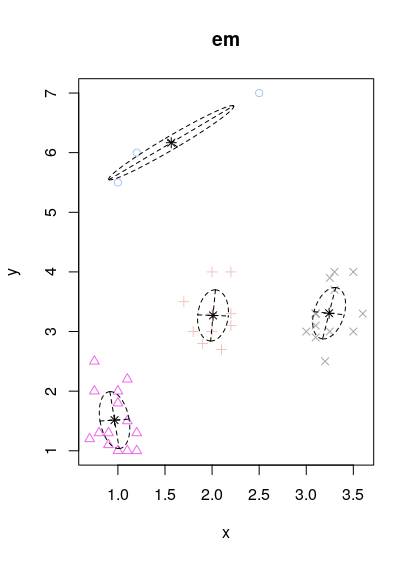
\includegraphics[scale=0.5]{EMplot.png}
\end{exercise}

		
		\begin{exercise}[p=3]{Noise}
		
			\textbf{K-Means}:\\
			K-Means does not treat noise seperately. Each point (including noise) is assigned to exactly one cluster.\\
				\begin{itemize}
				 \item \textbf{Uniform noise:} Depends on the ratio of noise. If there is significantly less noise than actual data points, the effect of the noise will be small. However with more noise, the cluster means will be significantly shifted by the influence of the noise, thereby deteriorating the quality of the clustering. Because the noise is uniformly distributed and affects all clusters similarily the effect wont be large.
				 \item \textbf{Non-uniform noise:} Blops of noise with many points might constitue an own cluster. If the noise is unevenly split among the clusters (, which is much more likley with a non-uniform distribution,) the mean values of the clusters can be significantly shifted and destroy the clustering.
				\end{itemize}
				
				
				\bigskip
						
			\textbf{Single-linkage}:\\
			Noise is indirectly classified, depending on the cutting level of the hierarchical clusters. The points, which have not been merged until the cutting point, constitute the noise cluster. Noise, which is in direct proximity of a cluster, will always be added to that cluster.
			\begin{itemize}
				 \item \textbf{Uniform noise:} If the noise is denser than some clusters, these clusters will vanish in the noise. Otherwise the noise is no problem.
				 \item \textbf{Non-uniform noise:} If there are some places with dense noise, they will be identified as a cluster. Furthermore even a very narrow chain (but relatively dense) can connect real clusters together.
			\end{itemize}
			
			\textbf{DBSCAN}:\\
			Less dense areas (depending on the parameters $\epsilon$ and minPoints) will be classified as noise.\\
			\begin{itemize}
				 \item \textbf{Uniform noise:} If the uniform noise is too dense for $\epsilon$ and minPoints, then everything will be identified as a single cluster. If the noise is less dense, no noise point will be classified as a core point, therefore most of the noise will be classified as noise. However some noise points might be recognized as boarder points of real clusters.
				 \item \textbf{Non-uniform noise:} Dense noise will be identified as clusters. However less dense noise will always be classified as such.
			\end{itemize}
			
			
		\end{exercise}
		
		\begin{exercise}[p=7]{Unknown Data}
		\end{exercise}
		
		
\end{ukon-infie}
\end{document}
